    % ----------------------------------------------------------------------
        \subsection{Ideale les}
            Okay daar zijn we dan, een hippe 9 pagina-'s later. Laten we beginnen aan wat mijn ideale les zou zijn. Voor mijn voorbeeld neem ik een les van 50 minuten. Dit is omdat de meeste middelbare scholen lessen van 50 minuten hanteren. 
            
            % — — — — — — — — — — — — — — — — — — — — — — — — — — — — — — — — — 
            \subsubsection{Les Inrichting}
                \paragraph{Voorbereiding}
                    We beginnen natuurlijk met de voorbereidingen. Want een goed begin is het halve werk. Plus, we hadden al eerder geconstateerd dat een goed voorbereid white board met zo veel mogelijk visuele aspecten zeer belangrijk was om de les ook visueel sterk te houden. Dus dit is waar ik zou beginnen. 

                    \bigskip

                    \noindent Allereerst moeten we een planning maken, als we deze maken kunnen we daarop verder bouwen. Het heeft geen zin als we 100 slides aan uitleg maken en maar 5 minuten er voor over houden. Dat is is een nieuwe slide elke 3 seconden. Het is belangrijk dat we onze planning SMART noteren, dit houd ons consistent, aanspreekbaar, en controleerbaar. Boven op dat het ons op schema houd, kan het zijn dat leerlingen nieuwsgierig worden. De leerlingen zijn dan onbewust actief het leer process aan het ondersteunen door hun zelf te motiveren en verwachtingen opstellen.\cite{NAME-ME}
                    
                    \bigskip

                    \noindent Hierna zou ik beginnen met een mind-map over het onderwerp en alles wat er aan gerelateerd is. \hyperlink{https://www.mindnode.com}{\underline{Mind Note}} is een fantastische app hiervoor. De subscription is een scam, maar de gratis versie werkt fantastisch. 
                    
                    \bigskip

                     \begin{center}
                        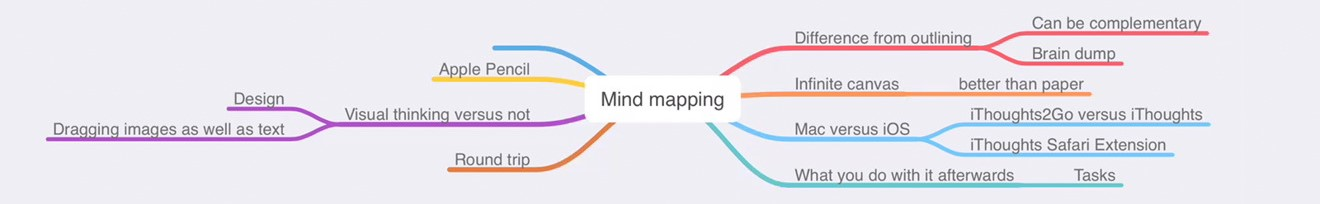
\includegraphics[width=35em]{Eindopdracht-Tygo-van-den-Hurk-1705709/Resources/Images/Mind-Note.jpg}
                    \end{center}
                    
                    \bigskip

                    \noindent Next, kunnen we beginnen aan de Dia-'s. Hierbij gebruiken we de Mind Note van eerder. Hiermee kunnen we gemakkelijk hoofdzaak van bij zaak scheiden. Nadat we dat gedaan hebben Passen we de een paar principes toe. We maken dingen dik gedrukt en gekleurd als het belangrijk is. Max een gekleurd ding op een slide. Afbeeldingen in plaats van woorden waar mogelijk. Lettertype is OpenDyslextic, uiteraard. Tot slot, een grote ergernis van mij, onderstreep het woord \underline{niet}. Ik lees zo vaak over dit woord heen, en ik weet dat een hoop dyslexten dit ook doen. Dit word is gewoon onzichtbaar, ik weet niet waarom.

                    \bigskip

                    \noindent Nu dat we ons white board, verhaal, en visuals voorbereid hebben zijn we klaar om de les te beginnen.
                    
                \paragraph{Terug halen van de voor kennis (5 minuten)}
                    We beginnen de les met het ophalen van de voorkennis. We moeten namelijk er voor zorgen dat de kennis die nodig is voor de uitleg van straks al klaar staat. Als ze niet weten wat een driehoek is, wens ik je veel succes met het uitleggen met wat een gelijkbenige driehoek is. We willen de voorkennis activeren door middel van het stellen van vragen. Het is belangrijk dat we positief blijven, en ons "samen" opstellen\cite{samen-boven-leads-to-better-results}. We willen ze niet afschrikken, of laten voelen alsof we ze aan het overhoren zijn. Het moet een soort van spel zijn. Dit helpt vooral mensen met ADHD. Mensen met ADHD leren veel sneller in spel vorm.\cite{ADHD-en-games}

                    Zodra een leerling antwoord geeft zijn d'r drie dingen die d'r kunnen gebeuren.
                    \begin{itemize}
                        \item{\textbf{Een, de leerling heeft het goed.}
                            Zodra een vraag goed is beantwoord herhalen we dit. Dit is belangrijk omdat het kan zijn dat er leerlingen afgeleid waren, of het oprecht niet hadden gehoord. Door middel van het goede antwoord te herhalen zorgen we d'r voor dat de leerlingen nóg een keer over heen gaan. We voegen er daarnaast ook een compliment aan toe. We willen ze belonen voor hun nek uit te steken. En we willen natuurlijk dit gedrag stimuleren. 
                        }
                        \item{\textbf{De leerling heeft de vraag half goed.}
                            We starten natuurlijk met het juiste te herhalen. Het foute herhalen we niet. Het juiste moet namelijk in hun hoofd blijven zitten. Daarna geven we een compliment omdat we dit het antwoord geven willen stimuleren. We vragen aan de klas of iemand anders kan helpen. Het is belangrijk dat we niet vragen of iemand anders het wel weet. Want dan zeggen we indirect dat de eerste leerling het fout had, en dat hadden we 'niet gehoord'. We vragen het alsof we samen een puzzel aan het oplossen zijn, en hulp nodig hebben. Dit houd de gedachte er in dat het een spelletje is. Daardoor ligt er geen druk op de leerlingen om het juist te hebben.\cite{games-help} En helpt het studenten leren door middel van trial-en-error.\cite{games-help}
                        }
                        \item{\textbf{De leerling zit d'r compleet naast.}
                            We beginnen met het zeggen waarom dit niet klopt en een hint naar het juiste antwoord. Daarna geven we natuurlijk een compliment. We vragen wederom of een student ons kan helpen met deze puzzel. Het is belangrijk positief te blijven.
                        }
                    \end{itemize}

                    \bigskip

                    \noindent De rede dat we de voorkennis herhalen is omdat het vaak opbrengen van iets lijd tot dat dat ding opgeslagen word in het lange termijn geheugen.\cite{repeating-leads-to-long-term-memory} Dus door het activeren van de voorkennis zorgen we er voor dat de les stof in het langer termijn geheugen komt. Precies waar we het willen hebben.
                        
                \paragraph{Uitleg (5 minuten + 5 in bruikleen)}
                    Nu dat we de voorkennis herhaald hebben is het belangrijk dat we hier op verder bouwen. We beginnen met duidelijk het les doel te herhalen. Het is namelijk belangrijk dat we de leerlingen activeren voor het belangrijkste stukje van de les. We vragen de leerlingen of ze dit concept al snappen, of zouden kunnen uitleggen. 

                    \bigskip
                    
                    \noindent Als een leerling een poging maakt geven we die een compliment en herhalen we het goede dat nog niet te ver is van de voorkennis. Als een leerling het helemaal goed uitlegde en het concept begreep geven we hem een zakje snoep. Waarom doen we dit? Nou, zoals ik al eerder zei, de les een een spelletje. En wat gebeurd er als je de jackpot scored op een game show? Dat klopt, dan krijg je een flinke beloning. 
                    
                    \bigskip
                    
                    \noindent Helaas kan ik geen 10 euro weg geven iedere keer, want zoveel krijg je als leraar niet betaald. Gelukkig hoeft dat ook niet. Een zakje snoep is een veel grotere beloning dan een compliment. Suiker geeft een grote lading dopamine vrij vergelijkbaar met drugs.\cite{sugar-equals-drugs} Ik ben geen voorstander om kinderen drugs te voeren. Maar dit ziet er veel belovend uit. Niet allen stimuleert het om complexe vraagstukken zelf al proberen op te lossen, het stimuleert leerlingen om zelf studie te doen en in het voren te werken. Ze weten namelijk dit onderwerp de volgende les behandeld word en dat dit studeren beloond word. 
                    
                    \bigskip
                    
                    \noindent Ongeacht wat de leerlingen antwoorden, leggen het concept uit. Maar afhankelijk van hoeveel leerlingen de vraag wilde/dacht te kunnen antwoorden krijgen we een schatting van hoeveel tijd leerlingen nodig hebben voor dit concept. Als niemand ook maar een poging kon maken is het duidelijk dat dit concept meer tijd nodig heeft. Dan nemen we de volle 10 minuten. Als iedereen het eigenlijk al wist dan hebben we maar 5 minuten nodig en kunnen we deze gebruiken in de vragen ronden. 
                    
                    \bigskip
                    
                    \noindent Mijn uitleg zal veel voorbeeld vragen bevatten. Waarom doe ik dit zo? Theorie is cool en al, maar zo leer je niet altijd. Nadat het concept is uitgelegd leg ik oppervlakkig de theorie uit. Leerlingen die de diepere theorie er achter willen weten happen toch wel. Die vragen dadelijk privé hoe het diepere stuk er uit zit. Wat doen we als ze zulke goede vragen stellen en graag in het diepere, moeilijkere stuk willen werken? That's right, jackpot, zakje Haribo voor de gelukkige. Dit willen we stimuleren en herbergen. Nieuwsgierigheid en enthousiasme. Dit geld ook voor leerlingen die het na de uitleg nog niet snapte en vroegen om extra uitleg. Dat is goed gedrag. We geven ze een complimentje, en zeggen dat ze het heel goed gedaan hebben. Daarna melden we de we volgende les terug komen en checken of de leerling het nog steeds snapt. Doen ze dit? Extra complimentje. Door er op terug te komen herhalen we het nog een keertje met de leerling en zorgen we er voor dat we gegarandeerd het juiste concept in het langer termijn geheugen van de leerling proppen.
                    
                \paragraph{Instructie (10 minuten)}
                    We beginnen de instructie met uitleggen wat het doel is van de instructie, en welke opdrachten we af gaan maken. Dan weten de leerlingen waar ze aan toe zijn en wat van ze verwacht wordt. Het doel van de instructie is dat ze inzien wat ze moeten doen om de stof die ze zojuist hebben geleerd to te passen. Daarom maken we ze de opdrachten eerst samen in de instructie. Zo heeft iedere leerling de kans om te zien hoe je met deze stof werkt.

                    \bigskip
                    
                    \noindent Een probleem dat veel voorkomt is dat de stof te snel word uitgelegd wanneer het lastig word. Daarom pas ik een automatische strategie toe waarbij ik persoonlijk geen moeite hoef te steken om het werkende te houden en niet alleen leerlingen het tempo bepalen maar ook zorgen dat de stof gegarandeerd duidelijk is. Dit doe ik door duidelijk te maken dat door vragen te stellen je me vertraagd. Dan hebben hun niet alleen de tijd om te begrijpen wat er gebeurd, maar ook de kans om te zorgen dat ze het snappen. Ik heb dit in de praktijk gezien door meerdere leraren, die dit met 100\% succes rate toepasten.\cite{succesfull-instructions} Zodra de leerlingen door hebben dat vragen stellen beter werkt dan het maar snel op te schrijven om er later op terug te komen.

                    \bigskip
                    
                    \noindent Iets heel belangrijks dat we moeten doen als we de instructie doen is het zorgen dat we elke keer andere studenten pakken. Als we dit niet doen krijg je dat die ene slimme student alle antwoorden geeft. 
                    
                \paragraph{Groepsopdracht (10 minuten)}
                    Deze vraag is moeilijker dan de vragen die ik zojuist met ze gemaakt heb en word gemaakt in paren en anders alleen. Dit is omdat je al snel krijgt dat twee het werk doen en de derde er bij zit. Als je het met z'n tweeën doet, heb je dat probleem niet. Als bonus heb je dat dit voor mensen die sociaal niet zo sterk zijn het nu makkelijker is om te oefenen. Success om tussen twee mensen te komen als je dit dood eng vind, niet sociaal bent, en niet eens zeker weet of je ideee wel goed is. Terwijl het voorstellen van een idee aan één persoon die verwacht dat jij ook input leverd en boom! Dat is een veel beter idee. Het helpt ook met mensen met autisme. Zei zijn vaak de minder sterke op een sociaal vlak. Ergens hierboven 5 pagina's terug had ik beschreven bij de autisme les-tips dat een-op-een opdrachten een hele goede oefening zijn voor mensen met autisme om te oefenen op sociaal vlak. Gezien zei vaak beter zijn in technische vakken verwacht ik dat de ander weet dat deze hiervan veel kan leren en zich vooral naar de gene met autisme zal kijken. Waardoor de gene met autisme een goede kans heeft om uit te leggen en te oefenen met zijn sociale skills. Ik vind het daarom ook totaal niet erg dat leerlingen niet onderling over niet stof gerelateerde dingen praten. Dit gaan ze namelijk toch wel doen. Zo kan ik zorgen dat de concentratie tank weer vol loopt terwijl ze ook bezig zijn met de stof.

                    \bigskip

                    \noindent Nadat de 5 minuten aan werken aan de opdracht, plus 5 minuten van leerlingen die met elkaar praten over zijn, gaan we de opdracht bespreken. Dit doen we weer samen klassicaal. Dit doen we alleen later. Eerst vraag ik alle leerlingen om hun antwoorden in te  leveren. Deze kijk ik na voor de meest gemaakte fouten. Deze behandel ik later.
                    
                    \bigskip

                    \noindent De opdracht die ze maken is een van de opdrachten die ik voor ze heb uitgekozen. Ik zou meerdere opdrachten uitkiezen die ze zouden kunnen maken en ze dan zelf laten kiezen. Omdat ze zelf mogen kiezen welke ze maken ontstaat er intrinsieke motivatie.\cite{NAME-ME} Dat zal leerlingen motiveren om de groepsopdracht te maken. Bovenop beloon ik ieder tweetal dat meer dan een opdracht maakt. Het vertonen van meer doen dat dat van je gevraagd word, word uiteraard beloond.
                    
                \paragraph{Zelfstandig werken (10 minuten)}
                    Ik geef ze 10 minuten om aan huiswerk te werken. Dit geeft mij de tijd om de groepsopdracht na te kijken. Vaak vinden leerlingen dit fijn omdat ze dan minder thuis hoeven te doen. Dit vergroot ook de kans dat ze het huiswerk thuis ook daadwerkelijk maken omdat er minder nog gedaan moet worden.\cite{more-homework-equals-bad} Dit helpt ook met het verminderen van de kans op ene amygdala-kaping.\cite{more-homework-equals-bad} 

                    \bigskip

                    \noindent Zoals ik al eerder had vermeld geef ik hier leerlingen de kans om hun koptelefoons te gebruiken. Dit geeft mensen met autisme die zich nu misschien moe voelen na deze grote hoeveelheid verplichte interacties met mede studenten de kans om van al deze prikkels bij te komen. Het geeft de mensen met ADHD een kans om hun concentratie bij te tanken door middel van alle stimulatie die de kop telefoon geeft. Bovendien zorgt het er voor dat de tank niet leeg loopt. Als je iemand met ADHD in een muis stille kamer neer zet waar die alleen moet werken zonder enige stimulatie gaat deze onrust veroorzaken. Daar kunnen mensen met ADHD niks aan doen, ze hebben gewoon stimulatie nodig. Door koptelefoons te gebruiken laten ze ook mede studenten met rust. Bovendien ervaren leerlingen het mogen luisteren naar muziek als belonen, waardoor ik meer "samen" uitstraal. Wat zorgt voor betere prestaties.\cite{samen-boven-leads-to-better-results}
                    
                \paragraph{Bespreken meest gemaakte Fouten tijdens Groepsopdracht (5 minuten)}
                    Nadat ik door de oplossingen van de groepsopdracht ben heen gegaan ben, heb ik een idee met wat de leelingen het meeste struggelen. Ik ga dan samen met ze de opdracht maken. Eerst bereid ik mijn white board voor door midddel van de opdracht zelf uit te werken tot en met de fout die het meeste gemaakt is. Dan maak een dia met de fout gekleurd zodat het duidelijk is dat dit speciaal is. Ik vraag de leerlingen dan wat hier niet klopt, en wat we anders kunnen doen. Dan ga ik naar de volgende dia waar de foute stap vervangen is door de goede. Nog steeds opvallend gemarkeerd. Hierdoor onthouden leerlingen deze veel gemaakte fout beter.\cite{Visual-Learners-are-the-most-common} De gene die deze fouten gemaakt hadden voelen zich wel aangesproken omdat ze weten dat het om hun fout gaat, maar omdat ze anoniem blijven is er geen kans dat er schaamte ontstaat. Dit voorkomt een amygdala-kaping, of een shutdown.\cite{more-homework-equals-bad}\cite{autisme-shutdowns} Omdat de leerlingen aan het reflecteren zijn of zij deze fout gemaakt hadden en of ze begrijpen hoe het wel moet vind een meta cognitieve leer activiteit plaats.\cite{NAME-ME}
                    
                \paragraph{reflectie (5 minuten)}
                    Als er tijd over is omdat de uitleg geen 10 minuten hoeft te zijn. Is er tijd over voor reflectie. Hier geven we de leerlingen een complimentje over wat ze deze keer goed gedaan hebben. Ik ben persoonlijk niet van de vlakke complimentjes zoals "Goed gewerkt vandaag!" omdat dit onpersoonlijk is, en fake aanvoelt. Ik zou mijn complimentje persoonlijker maken zoals dat ik het heel fijn vond hoe goed ze de instructie hadden mee gedaan. Niet alleen is een persoonlijker complimentje echter. Het helpt ook met het aanmaken van zelf vertrouwen van de leerling.\cite{compliments-how-to}

            % — — — — — — — — — — — — — — — — — — — — — — — — — — — — — — — — — 
            \subsubsection{Waarom dit een goede les in richting is}
                Mijn ideale les bestaat uit een sterkte afwisseling van leertheorieen en leeractiviteiten. Dit houd de leerlingen scherp en zorgt dat de leerlingen en zorgt dat de leerlingen hun concentratie tot de max kunnen gebruiken. Daar boven op wissel ik constant hoe de leerling zich moet opstellen tussen een passieve en een actieve houding. Ik vind dat de leerlingen veel vrijheid, complimenten, en stimulatie om verder te gaan krijgen wat in mijn optiek zorgt voor een goede leer omgeving waar de leerling de kans krijgt om op hun eigen tempo ver te gaan. Ik zou zegen dat ik tijdens de hele les ”samen-boven” uit straal. Wat voor leerlingen de ideale opstelling was.\cite{samen-boven-leads-to-better-results} Bovenop zorg ik voor strucuur en ondersteuning.

            % — — — — — — — — — — — — — — — — — — — — — — — — — — — — — — — — — 
            \subsubsection{Waarom dit ook goed werkt voor neurodivergente leerlingen}
                Over ondersteuning gesproken, hoe heb ik de neurodivergente leerlingen ondersteund? Dat was namelijk het hele doel van dit passie projectje. Ik zou zeggen dat ik dit goed gedaan heb. Ik bood visuele ondersteuning. Hield structuur en mezelf voorspelbaar. Bood voor 60\% van de les de tijd voor leerlingen om te vragen stellen. Gaf neurodivergente leerlingen een kans om in een veilige omgeving te werken aan hun zwakke punten. En tot slot speelde in op hun sterke punten. Hoewel ik geen PhD heb in hoe je neurodivergente leerlingen moet les geven vind ik dat dit een geslaagde zelf verzonnen bonus objectieve is en ben ik trots op de aanpassingen die ik heb gemaakt in vergelijking met de lessen die ik altijd heb gekregen.
            